\newpage
\subsection{Snubber}
Due to the fast-switching application of the MOSFET it will create transients which must be supressed. This can be done using an electrical snubber connected between the MOSFET's drain and source. The snubber consists of a resistor and a capacitor in series. The snubber is specified to the following values:
\begin{equation}
	\begin{split}
		C_{snubber} &= \SI{250}{\nano \farad}\\
		R_{snubber} &= \SI{22}{\ohm}
	\end{split}
\end{equation}
Furthermore it is rated to be able to handle alternating voltages up to \SI{250}{\volt} and DC-voltages up to \SI{630}{\volt} - which is more than enough for this application. As specified before, the snubber-circuit is placed between the MOSFET's drain and source.

\begin{figure}[H]
	\centering
	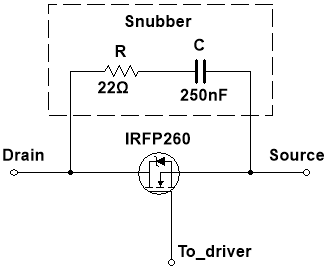
\includegraphics[width=0.5\linewidth]{Hardware/LoadSystem/Snubber}
	\caption{The placement of the snubber-circuit in the system}
	\label{fig:SnubberCircuit}
\end{figure}

When the snubber is inserted in the Load System it will be part of a filter consisting of the Generator, the Snubber and the Load. In order to determine ift the filter is stable, the damping ratio must be calculated. This can be done by using the values for the Generator's internal armature: 
\begin{equation}
	\begin{split}
		L_a &= \SI{0.072}{\milli \henry}\\
		R_a &= \SI{103}{\milli \ohm}\\
		R_{load} &= \SI{1.1065}{\ohm}
	\end{split}
\end{equation}

The filter can be modelled as seen on the the diagram below:
\begin{figure}[H]
	\centering
	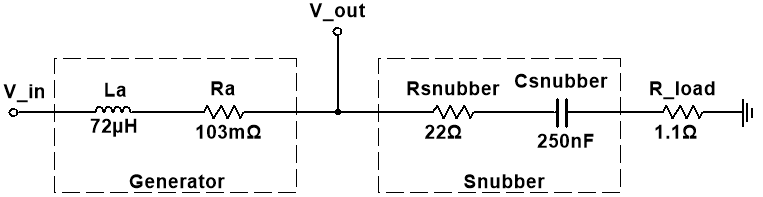
\includegraphics[width=0.9\linewidth]{Hardware/LoadSystem/SnubberFilter}
	\caption{The snubber's filter}
	\label{fig:SnubberFilter}
\end{figure}

The filter's transfer function in the s-domain can be found using the Laplace transform and standard circuit-analysis. The damping ratio can then be calculated as:
\begin{equation}
	\begin{split}
		\zeta &= \frac{(R_{snubber} + R_{load} + R_a) \cdot \sqrt{C_{snubber} \cdot  L_a}}{2 \cdot L_a}\\
		&= \frac{(\SI{22}{\ohm} + \SI{1.1065}{\ohm} + \SI{103}{\milli \ohm}) \cdot \sqrt{\SI{250}{\nano \farad} \cdot \SI{0.072}{\milli \henry}}}{2 \cdot \SI{0.072}{\milli \henry}}\\
		&= 0.683
	\end{split}
\end{equation}
As the damping ratio lies between 0 and 1 the system will be underdamped - but stable.